% !TEX root = ../main.tex

\section{Board and Signal Chain}
\label{sec:results-board}

The self-test reads the grounded and the reference input of both ADCs, then pulls every contact up and down with the jacks empty and checks that only the expected input follows. All 32 checks passed in \qty{1.02}{\second} on the first run, including the tip switch following the tip of every empty jack. The grounded inputs read \qty{1.3}{\milli\volt} and \qty{1.5}{\milli\volt}, the offset discussed below, and the reference inputs \qty{2.5000}{\volt}.

Ripple was measured AC-coupled at the test points of the input and of the three rails in four operating states, as the root-mean-square (RMS) average over 70 to 1000 acquisitions (\cref{fig:supply-ripple}). For the 7-bit value to stay stable, $\pm3\sigma$ of the ripple must fit within one step of the reference, $\qty{2.5}{\volt}/127 = \qty{19.7}{\milli\volt}$, which allows \qty{3.28}{\milli\volt} RMS. The ripple falls along the regulator chain and stays below the limit on every rail. The \qty{3.3}{\volt} and \qty{2.5}{\volt} rails stay at or just above the noise floor, with WiFi raising them visibly. The \qty{5}{\volt} rail shows short spikes of about \qty{16}{\milli\volt} peak-to-peak once the microcontroller runs, possibly from the switching regulator on the Pico~2~W.

\begin{figure}[tb]
  \centering
  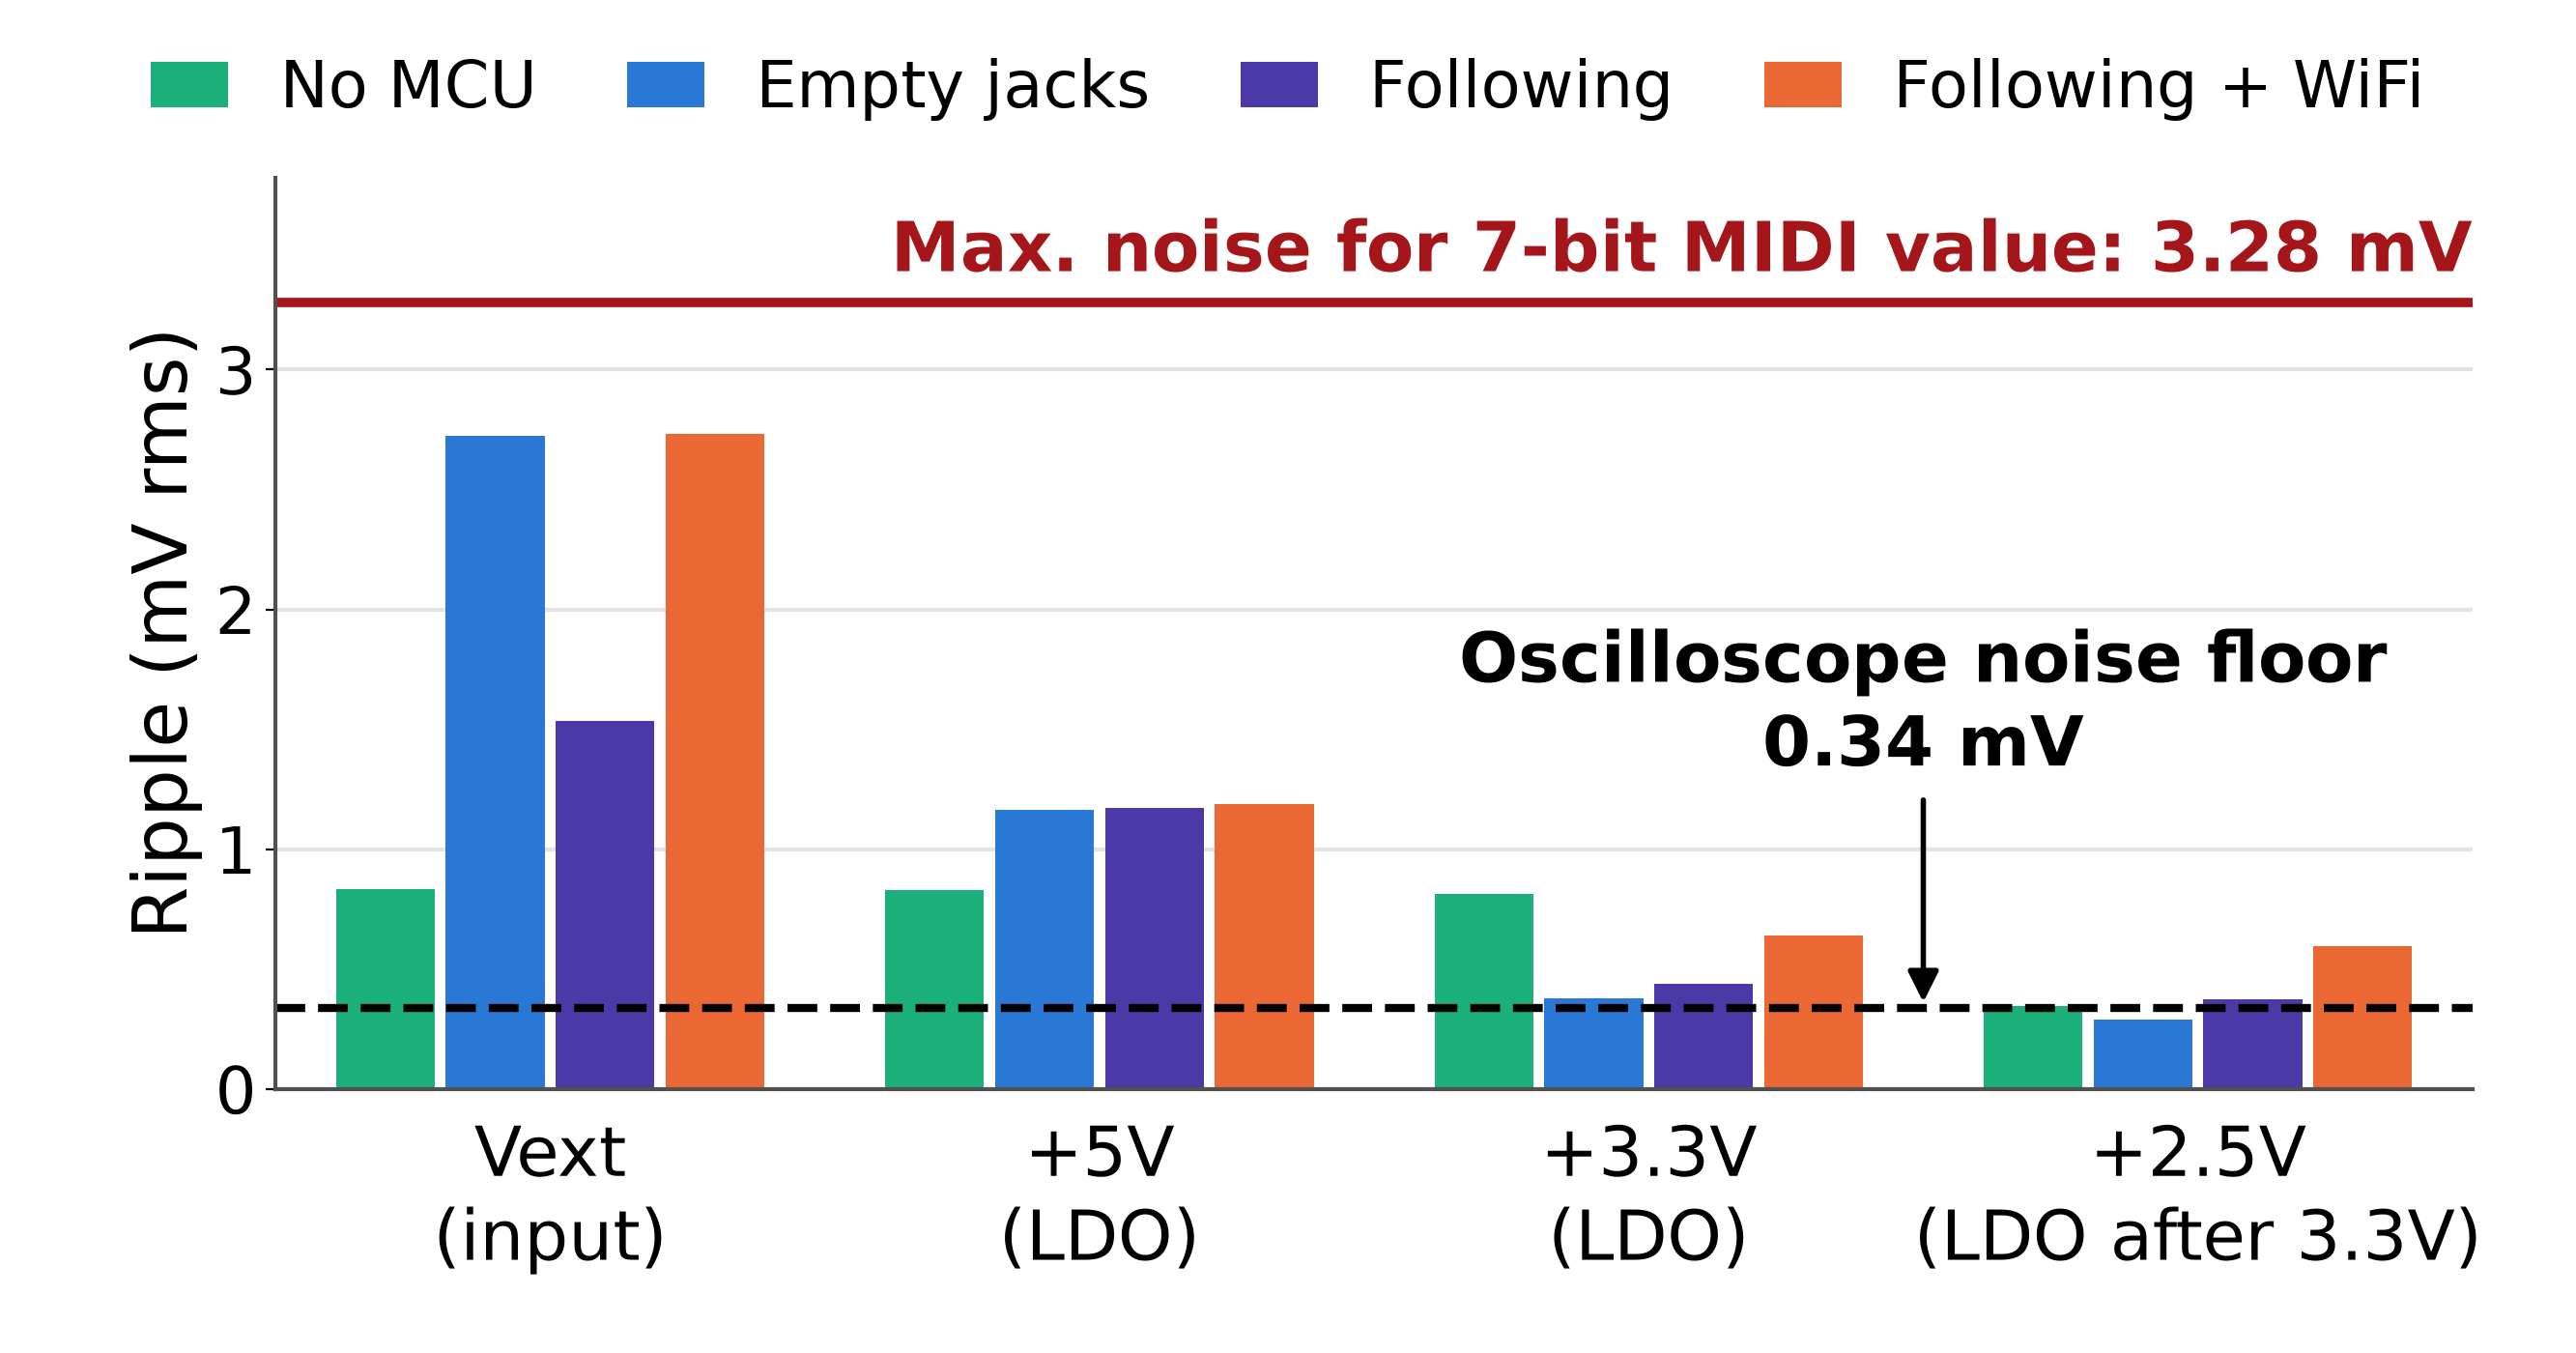
\includegraphics[width=0.56\linewidth]{05-results/figures/supply-rail-ripple}
  \titledcaption{Supply Rail Ripple}{RMS ripple of the input (Vext) and the regulated rails, AC-coupled at \qty{10}{\milli\second}/div, in four states: microcontroller removed (No MCU), empty jacks, one pedal followed, and the same with WiFi. Dashed: noise floor of the oscilloscope with the probe tip on ground. Red: limit for a stable 7-bit value.}
  \label{fig:supply-ripple}
\end{figure}

The SPI clock of \qty{3.95}{\mega\hertz} rises in \qty{10.2}{\nano\second} and the data in \qty{11.2}{\nano\second}, without ringing and with an overshoot below one vertical resolution step of the oscilloscope (\cref{fig:spi-edges}). On the empty board, the ADC noise was \qtyrange{15}{85}{\micro\volt} at \qty{315}{\hertz}, with a constant offset of about \qty{1.4}{\milli\volt} that the rail measurement removes (\cref{tab:adc-noise}).
